\documentclass[12pt]{article}
%%---------------------------------------------------------------------
% packages
% geometry
\usepackage{geometry}
% font
\usepackage{fontspec}
\defaultfontfeatures{Mapping=tex-text}  %%如果没有它,会有一些 tex 特殊字符无法正常使用,比如连字符。
\usepackage{xunicode,xltxtra}
\usepackage[BoldFont,SlantFont,CJKnumber,CJKchecksingle]{xeCJK}  % \CJKnumber{12345}: 一万二千三百四十五
\usepackage{CJKfntef}  %%实现对汉字加点、下划线等。
\usepackage{pifont}  % \ding{}
% math
\usepackage{amsmath,amsfonts,amssymb}
% color
\usepackage{color}
\usepackage{xcolor}
\definecolor{EYE}{RGB}{199,237,204}
\definecolor{FLY}{RGB}{128,0,128}
\definecolor{ZHY}{RGB}{139,0,255}
% graphics
\usepackage[americaninductors,europeanresistors]{circuitikz}
\usepackage{tikz}
\usetikzlibrary{positioning,arrows,shadows,shapes,calc,mindmap,trees,backgrounds}  % placements=positioning
\usepackage{graphicx}  % \includegraphics[]{}
\usepackage{subfigure}  %%图形或表格并排排列
% table
\usepackage{colortbl,dcolumn}  %% 彩色表格
\usepackage{multirow}
\usepackage{multicol}
\usepackage{booktabs}
% code
\usepackage{fancyvrb}
\usepackage{listings}
% title
\usepackage{titlesec}
% head/foot
\usepackage{fancyhdr}
% ref
\usepackage{hyperref}
% pagecolor
\usepackage[pagecolor={EYE}]{pagecolor}
% tightly-packed lists
\usepackage{mdwlist}

\usepackage{styles/iplouccfg}
\usepackage{styles/zhfontcfg}
\usepackage{styles/iplouclistings}

%%---------------------------------------------------------------------
% settings
% geometry
\geometry{left=2cm,right=1cm,top=2cm,bottom=2cm}  %设置 上、左、下、右 页边距
\linespread{1.5} %行间距
% font
\setCJKmainfont{Adobe Kaiti Std}
%\setmainfont[BoldFont=Adobe Garamond Pro Bold]{Apple Garamond}  % 英文字体
%\setmainfont[BoldFont=Adobe Garamond Pro Bold,SmallCapsFont=Apple Garamond,SmallCapsFeatures={Scale=0.7}]{Apple Garamond}  %%苹果字体没有SmallCaps
\setCJKmonofont{Adobe Fangsong Std}
% graphics
\graphicspath{{figures/}}
\tikzset{
    % Define standard arrow tip
    >=stealth',
    % Define style for boxes
    punkt/.style={
           rectangle,
           rounded corners,
           draw=black, very thick,
           text width=6.5em,
           minimum height=2em,
           text centered},
    % Define arrow style
    pil/.style={
           ->,
           thick,
           shorten <=2pt,
           shorten >=2pt,},
    % Define style for FlyZhyBall
    FlyZhyBall/.style={
      circle,
      minimum size=6mm,
      inner sep=0.5pt,
      ball color=red!50!blue,
      text=white,},
    % Define style for FlyZhyRectangle
    FlyZhyRectangle/.style={
      rectangle,
      rounded corners,
      minimum size=6mm,
      ball color=red!50!blue,
      text=white,},
    % Define style for zhyfly
    zhyfly/.style={
      rectangle,
      rounded corners,
      minimum size=6mm,
      ball color=red!25!blue,
      text=white,},
    % Define style for new rectangle
    nrectangle/.style={
      rectangle,
      draw=#1!50,
      fill=#1!20,
      minimum size=5mm,
      inner sep=0.1pt,}
}
\ctikzset{
  bipoles/length=.8cm
}
% code
\lstnewenvironment{VHDLcode}[1][]{%
  \lstset{
    basicstyle=\footnotesize\ttfamily\color{black},%
    columns=flexible,%
    framexleftmargin=.7mm,frame=shadowbox,%
    rulesepcolor=\color{blue},%
%    frame=single,%
    backgroundcolor=\color{yellow!20},%
    xleftmargin=1.2\fboxsep,%
    xrightmargin=.7\fboxsep,%
    numbers=left,numberstyle=\tiny\color{blue},%
    numberblanklines=false,numbersep=7pt,%
    language=VHDL%
    }\lstset{#1}}{}
\lstnewenvironment{VHDLmiddle}[1][]{%
  \lstset{
    basicstyle=\scriptsize\ttfamily\color{black},%
    columns=flexible,%
    framexleftmargin=.7mm,frame=shadowbox,%
    rulesepcolor=\color{blue},%
%    frame=single,%
    backgroundcolor=\color{yellow!20},%
    xleftmargin=1.2\fboxsep,%
    xrightmargin=.7\fboxsep,%
    numbers=left,numberstyle=\tiny\color{blue},%
    numberblanklines=false,numbersep=7pt,%
    language=VHDL%
    }\lstset{#1}}{}
\lstnewenvironment{VHDLsmall}[1][]{%
  \lstset{
    basicstyle=\tiny\ttfamily\color{black},%
    columns=flexible,%
    framexleftmargin=.7mm,frame=shadowbox,%
    rulesepcolor=\color{blue},%
%    frame=single,%
    backgroundcolor=\color{yellow!20},%
    xleftmargin=1.2\fboxsep,%
    xrightmargin=.7\fboxsep,%
    numbers=left,numberstyle=\tiny\color{blue},%
    numberblanklines=false,numbersep=7pt,%
    language=VHDL%
    }\lstset{#1}}{}
% pdf
\hypersetup{pdfpagemode=FullScreen,%
            pdfauthor={Haiyong Zheng},%
            pdftitle={Title},%
            CJKbookmarks=true,%
            bookmarksnumbered=true,%
            bookmarksopen=false,%
            plainpages=false,%
            colorlinks=true,%
            citecolor=green,%
            filecolor=magenta,%
            linkcolor=cyan,%red(default)
            urlcolor=cyan}
% section
%http://tex.stackexchange.com/questions/34288/how-to-place-a-shaded-box-around-a-section-label-and-name
\newcommand\titlebar{%
\tikz[baseline,trim left=3.1cm,trim right=3cm] {
    \fill [cyan!25] (2.5cm,-1ex) rectangle (\textwidth+3.1cm,2.5ex);
    \node [
        fill=cyan!60!white,
        anchor= base east,
        rounded rectangle,
        minimum height=3.5ex] at (3cm,0) {
        \textbf{\thesection.}
    };
}%
}
\titleformat{\section}{\Large\bf\color{blue}}{\titlebar}{0.1cm}{}
% head/foot
\setlength{\headheight}{15pt}
\pagestyle{fancy}
\fancyhf{}

\chead{\color{black!50!green}Assignment \#2}

\lfoot{\color{blue!50!green}Zhao Haiwei}
\cfoot{\color{blue!50!green}\href{http://vision.ouc.edu.cn/~zhenghaiyong}{CVBIOUC}}
\rfoot{\color{blue!50!green}$\cdot$\ \thepage\ $\cdot$}
\renewcommand{\headrulewidth}{0.4pt}
\renewcommand{\footrulewidth}{0.4pt}

%%---------------------------------------------------------------------
\begin{document}
%%---------------------------------------------------------------------
%%---------------------------------------------------------------------
% \titlepage
\title{\vspace{-2em}CV2015Spring---Assignment \#\textbf{2}\\
\normalsize{Due: Thursday, Apr 30 10:00 AM}}
\author{Zhao Haiwei}
\date{\vspace{-0.7em}Apr 16, 2015\vspace{-0.7em}}
%%---------------------------------------------------------------------
\maketitle\thispagestyle{fancy}
%%---------------------------------------------------------------------
\maketitle
%\tableofcontents 


%\section{Programming problem: salient object detection}
\section{Assignment requirement}

For this assignment, you will implement a version of the Object Detection technique. See Figure~\ref{fig:example} for an example.

\begin{figure}[!ht]
  \centering 
  \subfigure[]{ 
    \label{fig:example:a} %% label for first subfigure 
    \includegraphics[height=0.15\textheight]{object}} 
  \subfigure[]{ 
    \label{fig:example:b} %% label for second subfigure 
    \includegraphics[height=0.15\textheight]{scene}} 
  \subfigure[]{ 
    \label{fig:example:c} %% label for second subfigure 
    \includegraphics[height=0.15\textheight]{Result}} 
  \caption{Object detection.}
  \label{fig:example} %% label for entire figure 
\end{figure}

Your method must be Featuers2D-based, and at least one kind of Feature2D\footnote{Please refer to \url{http://docs.opencv.org/modules/features2d/doc/features2d.html}.} and matching strategy should be used. I will give you some tips for the implementation in the following sections.

\section{Tips}

The whole framework of the implementation for object detection is shown in Figure~\ref{fig:framework}, it may serve as a reference for your assignment. Next, I will introduce the implementation and requirement of each part of the framework for you.

\begin{figure}[!ht]
\centering
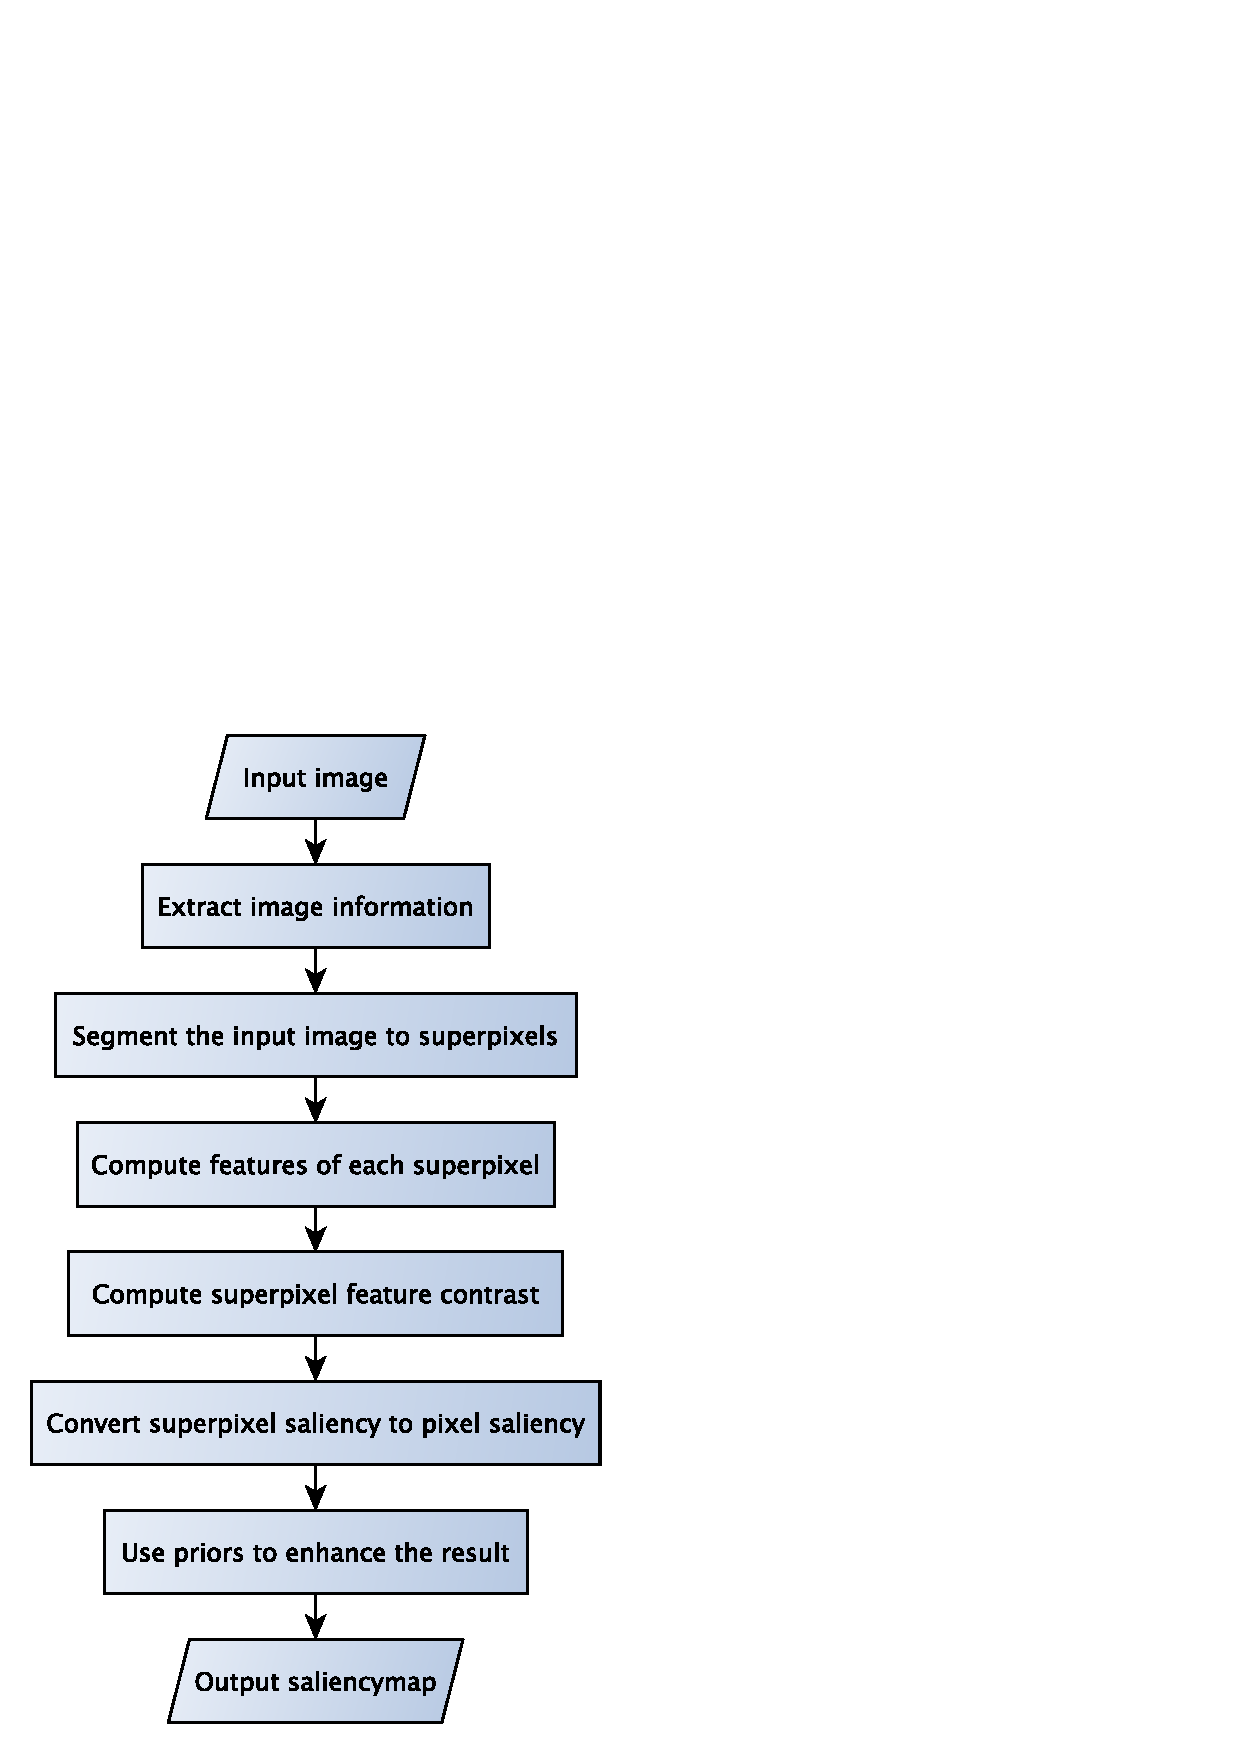
\includegraphics[height=0.6\textheight]{framework.png}
\caption{Framework of the implementation for object detection.}
\label{fig:framework}
\end{figure}

\subsection{Step 1: Input image}

The object image and scene image is given. Firstly, you should input the two images.

\subsection{Step 2: Color space conversion (5 points)}

\begin{description}
\item[Input] The input color image ($m \times n \times 3$ matrix), $m$ is the width of the input image, $n$ is the height of the input image.
\item[Output] $m \times n$ matrix. 
\item[Implementation] This step determines the kind of color space you want to use in step 2, and you should converse the color space from RGB to GRAY.
\end{description}

\subsection{Step 3: Features2D detection (15 points)}

\begin{description}
\item[Input] The gray image ($m \times n \times 1$ matrix), $m$ is the width of the input image, $n$ is the length of the input image. 
\item[Output]  Keypoints of object image and scene image. 
\item[Implementation] Detect the keypoints using Features2D Detector and store the result.
\item[Hint] There are lots of Features2D detection algorithms, such as SIFT, SURF, and so on. You can choose one of them which is fast and easy to implement.
\begin{figure}[!ht]
  \centering 
  \subfigure[]{ 
    \label{fig:Features2D:a} %% label for first subfigure 
    \includegraphics[height=0.15\textheight]{Feature_Detection_Result_a.jpg}} 
  \subfigure[]{ 
    \label{fig:Features2D:b} %% label for second subfigure 
    \includegraphics[height=0.15\textheight]{Feature_Detection_Result_b.jpg}} 
  \caption{Features2D detection.}
  \label{fig:Features2D} %% label for entire figure 
\end{figure}
\end{description}

\subsection{Step 4: Calculate descriptors (15 points)}

\begin{description}
\item[Input] The gray image ($m \times n \times 1$ matrix), $m$ is the width of the input image, $n$ is the length of the input image.The keypoints detected in Step 3.
\item[Output] One matrix describes the keypoints in the object image and one matrix describes the keypoints in the scene image.
\item[Implementation] Descriptors of the keypoints in the object image are stored in one Matrix and descriptors of the keypoints in the scene image are stored in another Matrix.
\end{description}

\subsection{Step 5: Match descriptors (20 points)}

\begin{description}
\item[Input] One matrix describes the keypoints in the object image and one matrix describes the keypoints in the scene image.
\item[Output] $M$ good matched keypoints between object image and scene image.
\item[Implementation] \mbox{}
\begin{itemize}
\item Step 5-1: You should quick calculate $x \times y$ ($x$, $y$ are the number of keypoints) distances (value) between keypoints, each value indicates the similarity of one keypoint from object image and one keypoint from scene image.
\item Step 5-2: Fix one keypoint from object image and select the min or max distance between the keypoint and one keypoint from scene image to find the best match,then change the fixed keypoint and do the same.
\item Step 5-3: You should draw only ``good'' matches (i.e. whose distance is less than $3*\min(distance)$).
\end{itemize}   
\item[Hint] There are lots of distance calculation algorithms, such as Hausdorff Distance, Euclidean Distance, and so on. You can choose one of them to calculate the similarity between two keypoints and find the best match.
\begin{figure}[!ht]
  \centering 
  \subfigure[]{ 
    \label{fig: result: a} %% label for first subfigure 
    \includegraphics[height=0.3\textheight]{Featur_FlannMatcher_Result.jpg}} 
  \subfigure[]{ 
    \label{fig: result: b} %% label for second subfigure 
    \includegraphics[height=0.3\textheight]{Feature_FlannMatcher_Keypoints_Result.jpg}} 
  \caption{Match descriptors.}
  \label{fig: Match descriptors} %% label for entire figure 
\end{figure}
\end{description}

\subsection{Step 6: Find homography transformation (20 points)}

\begin{description}
\item[Input] Keypoints of object image and scene image.
\item[Output] Matrix of homography transformation between two different point sets.
\item[Implementation] \mbox{}
\begin{itemize}
\item Step 6-1: Get $N$ keypoints from the good matches and store them in two different point sets.
\item Step 6-2: Calculate the matrix of homography transformation between the two different point sets.
\end{itemize} 
\item[Hint] There are lots of mapping transformation algorithms, I recommend you to use homography transformation.
\end{description}

\subsection{Step 7: Perspective transform (20 points)}

\begin{description}
\item[Input] Four corners of object image.
\item[Output] Four points of scene image which are corresponding to the four corners.
\item[Implementation] You can use the matrix of homography transformation which was got in Step 6 to perspective transform the four corners of object image to four points of scene image.
\end{description}

\subsection{Step 8: Localize the object (5 points)}

\begin{description}
\item[Input] The scene image which has four points (the mapped object in the scene image).
\item[Output] The matrix box in the scene image which contains the object in object image.
\item[Implementation] Draw lines between the four points (the mapped object in the scene image).
\begin{figure}[!ht]
\centering
\includegraphics[height=0.3\textheight]{Result.jpg}
\caption{Localize the object.}
\label{fig:localize}
\end{figure}
\end{description}


\section{Submission instructions}

\subsection{What to hand in?}

\begin{itemize}
\item Your matlab code or C/C++ code (show the result of each step in your code)
\item A ``Readme'' file to illustrate how to run your code
\item A report containing the following items:
\begin{itemize}
\item The title and your name at the top
\item A brief explanation of your implementation strategy corresponding to each step (in English)
\end{itemize}
\end{itemize}

\subsection{Where to hand in?}

Submit to Piazza in form of a followup below my assignment note.





%\bibliographystyle{plain}
%
%\bibliography{Assignment1} 

%%---------------------------------------------------------------------
\end{document}
